% Created 2019-03-26 Tue
% Intended LaTeX compiler: pdflatex
\documentclass[11pt, reqno, oneside]{amsbook}
              \newcommand\subtitle[1]{\newcommand\mrgsubtitle{#1}}
\newcommand\mrgproject{Torsten}
\newcommand\mrgtitle{Torsten: A Pharmacokinetic/Pharmacodynamic Model Library for Stan}
\newcommand\mrgsubtitle{\Large{User Manual} \linebreak (Torsten Version 0.85, Stan version 2.18.0)}
\renewcommand\maketitle{
  \begin{titlepage}%
    \definecolor{MRGGreen}{rgb}{0, 0.350, 0.200}

    \thispagestyle{empty}

    \begin{center}
      
\includegraphics[height=0.75in]{graphics/logo.jpg}\\
      \vspace{10mm} %5mm vertical space
      \textcolor{MRGGreen}{\sf Metrum Research Group LLC \hfill 2 Tunxis Road, Suite 112} \\
      \textcolor{MRGGreen}{\sf Phone: 860.735.7043 \hfill Tariffville, CT 06081}\\
      \textcolor{MRGGreen}{\sf billg@metrumrg.com, yiz@metrumrg.com \hfill \href{http://www.metrumrg.com/}{www.metrumrg.com}}\\
      {\Huge \textcolor{MRGGreen}{\textbf{\mrgproject}} \\ \ \\  \huge{\mrgtitle} \\ \ \\ \mrgsubtitle\\ \ \\ \ \\
        
        \large May 2019}
    \end{center}

    \clearpage
  \end{titlepage}%
}

\usepackage{imakeidx}
\makeindex
\usepackage[letterpaper, width=6.5in, height=9in]{geometry}
\usepackage{graphicx}
\usepackage{pdfpages}
\usepackage{amssymb}
\usepackage{epstopdf}
\usepackage{xcolor}
\definecolor{MRGGreen}{rgb}{0, 0.350, 0.200}
\usepackage[colorlinks=true, citecolor=MRGGreen, urlcolor=MRGGreen, linkcolor=MRGGreen]{hyperref}
\usepackage{courier}
\usepackage{listings}
\usepackage{siunitx}
\usepackage{booktabs}
\usepackage[framemethod=TikZ, skipabove=10pt, skipbelow=10pt, backgroundcolor=black!5, roundcorner=4pt, linewidth=1pt]{mdframed}
\BeforeBeginEnvironment{minted}{\begin{mdframed}}
\AfterEndEnvironment{minted}{\end{mdframed}}
\usepackage{subcaption}
\renewcommand{\chaptername}{}
\numberwithin{equation}{chapter}
\numberwithin{figure}{chapter}
\numberwithin{table}{chapter}
\usepackage[section]{placeins}
\theoremstyle{remark}
\newtheorem{example}{Example}
\newtheorem{remark}{Remark}


\usepackage[utf8]{inputenc}
\usepackage[T1]{fontenc}
\usepackage{graphicx}
\usepackage{grffile}
\usepackage{longtable}
\usepackage{wrapfig}
\usepackage{rotating}
\usepackage[normalem]{ulem}
\usepackage{amsmath}
\usepackage{textcomp}
\usepackage{amssymb}
\usepackage{capt-of}
\usepackage{hyperref}
\usepackage[newfloat]{minted}
\usepackage{caption}
\setcounter{secnumdepth}{3}
\author{Yi Zhang}
\date{\today}
\title{Torsten: A Pharmacokinetic/Pharmacodynamic Model Library for Stan\\\medskip
\large User Manual \\  (Torsten Version 0.85, Stan version 2.18.0)}
\hypersetup{
 pdfauthor={Yi Zhang},
 pdftitle={Torsten: A Pharmacokinetic/Pharmacodynamic Model Library for Stan},
 pdfkeywords={},
 pdfsubject={},
 pdfcreator={Emacs 25.3.1 (Org mode 9.1.3)}, 
 pdflang={English}}
\begin{document}

\maketitle
\tableofcontents


\section*{Development team}
\label{sec:orgba15e9f}
\subsection*{Bill Gillespie}
\label{sec:org365cdab}
\href{mailto:billg@metrumrg.com}{\texttt{billg@metrumrg.com}},
Metrum Research Group, LLC
\subsection*{Yi Zhang}
\label{sec:orga82e59c}
\href{mailto:yiz@metrumrg.com}{\texttt{yiz@metrumrg.com}}, Metrum Research Group, LLC
\subsection*{Charles Margossian}
\label{sec:org62552bb}
\noindent
\href{mailto:charles.margossian@columbia.edu}{\texttt{charles.margossian@columbia.edu}}, Columbia University, \\
\hspace*{0.5cm} Department of Statistics (formerly Metrum Research Group, LLC)

\chapter*{Acknowledgements}
\label{sec:org99d4b11}
\section*{Institutions}
\label{sec:orge6a0e3f}
We thank Metrum Research Group, Columbia University, and AstraZeneca.
\section*{Funding}
\label{sec:org1ce2b16}
This work was funded in part by the following organizations:
\subsection*{Office of Naval Research (ONR) contract N00014-16-P-2039}
\label{sec:org2d07e64}
provided as part of the Small Business Technology Transfer (STTR)
program. The content of the information presented in this document
does not necessarily reflect the position or policy of the
Government and no official endorsement should be inferred.
\subsection*{Bill \& Melinda Gates Foundation.}
\label{sec:orgdd7196b}
\section*{Individuals}
\label{sec:org8648219}
We thank the Stan Development Team for giving us guidance on how to
create new Stan functions and adding features to Stan's core language
that facilitate building ODE-based models.

We also thank Kyle Baron and Hunter Ford for helpful advice on coding
in C++ and using GitHub, Curtis Johnston for reviewing the User
Manual, and Yaming Su for using Torsten and giving us feedback.

\chapter{Introduction}
\label{sec:orgc05530e}
Stan is an open source probabilistic programing language designed
primarily to do Bayesian data analysis \cite{carpenter17_stan}. Several of its
features make it a powerful tool to specify and fit complex models. 
First, its language is very expressive and flexible.
Secondly, it implements a variant of the No U-Turn Sampler (NUTS),
an adaptive Hamiltonian Monte Carlo algorithm, which was proven
more efficient than commonly used Markov chains Monte Carlo (MCMC)
sampler for high dimensional problems 
\cite{hoffman_no-u-turn_2014, betancourt_hmc_2018}.
%
Our goal is to harness these innovative features and make Stan a better
software for pharmacometrics modeling. Our efforts are twofold:
\begin{enumerate}
\item We contribute to the development of features, such as functions that support differential equations based models, and implement them directly into Stan's core language.
\item We develop Torsten, an extension with specialized pharmacometrics functions.
\end{enumerate}

Throughout the process, we work very closely with the Stan Development
Team. 
We have benefited immensely from their mentorship, advice, and
feedback. Just like Stan, Torsten is an open source project that
fosters collaborative work. Interested in contributing? Shoot us an
e-mail and we will help you help us (\href{mailto:billg@metrumrg.com}{billg@metrumrg.com})!

Torsten is licensed under the BSD 3-clause license.

\begin{mdframed}
\textbf{WARNING:} The current version of Torsten is a \emph{prototype}. It
is being released for review and comment, and to support limited
research applications. It has not been rigorously tested and should
not be used for critical applications without further testing or
cross-checking by comparison with other methods.

We encourage interested users to try Torsten out and are happy to
assist. Please report issues, bugs, and feature requests on
\href{https://github.com/metrumresearchgroup/stan}{our GitHub page}.
\end{mdframed}

\section{Overview}
\label{sec:orgb30183b}
Torsten is a collection of Stan functions to facilitate analysis of
pharmacometric data using Stan. The current version
includes:
\begin{itemize}
\item Specific linear compartment models:
\begin{itemize}
\item One compartment model with first order absorption.
\item Two compartment model with elimination from and first order absorption into central compartment
\end{itemize}
\item General linear compartment model described by a system of first-order \underline{linear} Ordinary Differential Equations (ODEs).
\item General compartment model described by a system of first order ODEs.
\item Mix compartment model with PK forcing function described by a linear one or two compartment model.
\end{itemize}

The models and data format are based on
NONMEM\textregistered{}\footnote{NONMEM\textregistered{} is licensed and distributed by ICON Development Solutions.}/NMTRAN/PREDPP
conventions including:
\begin{itemize}
\item Recursive calculation of model predictions
\begin{itemize}
\item This permits piecewise constant covariate values
\end{itemize}
\item Bolus or constant rate inputs into any compartment
\item Handles single dose and multiple dose histories
\item Handles steady state dosing histories
\begin{itemize}
\item Note: The infusion time must be shorter than the inter-dose interval.
\end{itemize}
\item Implemented NMTRAN data items include: TIME, EVID, CMT, AMT, RATE, ADDL, II, SS
\end{itemize}

In general, all real variables may be passed as model parameters. A
few exceptions apply to functions which use a numerical
integrator (i.e. the general and the mix compartment
models). The below listed cases present technical difficulties, which we expect to
overcome in Torsten's next release:
\begin{itemize}
\item In the case of a multiple truncated infusion rate dosing regimen:
\begin{itemize}
\item The bioavailability (F) and the amount (AMT) must be fixed.
\end{itemize}
\end{itemize}

This library provides Stan language functions that calculate amounts
in each compartment, given an event schedule and an ODE system.

\section{Implementation summary}
\label{sec:org380dc5f}
\begin{itemize}
\item Current v0.85 Torsten is based on Stan v2.18.0.
\item All functions are programmed in C++ and are compatible
with the Stan math automatic differentiation library \cite{carpenter15_stan_math_librar}
\item One and two compartment models are based on analytical solutions of governing ODEs.
\item General linear compartment models are based on semi-analytical solutions using the built-in matrix exponential function
\item General compartment models are solved numerically using built-in ODE integrators in Stan. The tuning parameters of the solver are adjustable. The steady state solution is calculated using a numerical algebraic solver.
\item A mix compartment model's PK forcing function is solved
analytically, and its forced ODE system is solved
numerically.
\end{itemize}

\section{Development plans}
\label{sec:org966fbf1}
Our current plans for future development of Torsten include the
following:
\begin{itemize}
\item Build a system to easily share packages of Stan functions
(written in C++ or in the Stan language)
\item Allow numerical methods to handle
bioavailability fraction (F) as parameters in all cases.
\item Optimize Matrix exponential functions
\begin{itemize}
\item Function for the action of Matrix Exponential on a vector
\item Hand-coded gradients
\item Special algorithm for matrices with special properties
\end{itemize}
\item Fix issue that arises when computing the adjoint of the lag time
parameter (in a dosing compartment) evaluated at \(t_{\text{lag}} = 0\).
\item Extend formal tests
\begin{itemize}
\item We want more C++ Google unit tests to address cases users may
encounter
\item Comparison with simulations from the R package
\texttt{mrgsolve} and the software NONMEM\textregistered{}
\item Recruit non-developer users to conduct beta testing
\end{itemize}
\end{itemize}

\section{Changelog}
\label{sec:org1ae8c06}
\subsection{0.85 \textit{<2018-10-20 Sat>}}
\label{sec:org81fca5c}
\begin{itemize}
\item Added
\label{sec:org9a969ec}
\begin{itemize}
\item Dosing rate as parameter
\end{itemize}
\item Changed
\label{sec:orga13d796}
\begin{itemize}
\item Update with Stan version 2.18.0.
\end{itemize}
\end{itemize}

\subsection{0.84 \textit{<2018-02-24 Sat>}}
\label{sec:org3064cbb}
\begin{itemize}
\item Added
\label{sec:org2ff976f}
\begin{itemize}
\item Piecewise linear interpolation function.
\item Univariate integral functions.
\end{itemize}

\item Changed
\label{sec:orgd3bd3c1}
\begin{itemize}
\item Update with Stan version 2.17.1.
\item Minor revisions to User Manual.
\item Bugfixes.
\end{itemize}
\end{itemize}

\subsection{0.83 \textit{<2017-08-02 Wed>}}
\label{sec:org4a7cdf0}
\begin{itemize}
\item Added
\label{sec:orgc26a125}
\begin{itemize}
\item Work with TorstenHeaders
\item Each chain has a different initial estimate
\end{itemize}

\item Changed
\label{sec:org14893f4}
\begin{itemize}
\item User manual
\item Fix misspecification in ODE system for TwoCpt example.
\item Other bugfixes
\end{itemize}
\end{itemize}


\subsection{0.82 \textit{<2017-01-29 Sun>}}
\label{sec:org71a3795}
\begin{itemize}
\item Added
\label{sec:org10ec6bb}
\begin{itemize}
\item Allow parameter arguments to be passed as 1D or 2D arrays
\item More unit tests
\item Unit tests check automatic differentiation against finite differentiation.
\end{itemize}

\item Changed
\label{sec:orgaaf62c6}
\begin{itemize}
\item Split the parameter argument into three arguments: pMatrix
(parameters for the ODEs -- note: for linOdeModel, pMatrix
is replaced by the constant rate matrix K), biovar
(parameters for the biovariability), and tlag (parameters
for the lag time).
\item bugfixes
\end{itemize}
\end{itemize}

\subsection{0.81 \textit{<2016-09-27 Tue>}}
\label{sec:org666091e}
\begin{itemize}
\item Added
\label{sec:org715546a}
linCptModel (linear compartmental model) function
\end{itemize}

\subsection{0.80a \textit{<2016-09-21 Wed>}}
\label{sec:org90e24d2}
\begin{itemize}
\item Added
\label{sec:org5b05b62}
check\_finite statements in pred\_1 and pred\_2 to reject metropolis proposal if initial conditions are not finite
\end{itemize}




\chapter{Installation}
\label{sec:org3d2fe5d}
We are working with Stan development team to create a
system to add and share Stan packages. In the mean time,
the current repo contains forked version of Stan with
Torsten. The latest version of Torsten (v0.85) is
compatible with Stan v2.18.0. Torsten is agnostic to which
Stan interface you use. Here we provide command line and R
interfaces.

After downloading the project 

\begin{itemize}
\item \url{https://github.com/metrumresearchgroup/Torsten}
\end{itemize}

to \texttt{torsten\_path}, set the envionment variable
\mintinline[breaklines=true,fontsize=\footnotesize,breakanywhere=true]{sh}{TORSTEN_PATH} as
\begin{minted}[breaklines=true,fontsize=\footnotesize,breakanywhere=true]{sh}
# in bash
export TORSTEN_PATH=torsten_path
# in csh
setenv TORSTEN_PATH torsten_path
\end{minted}

\subsection{Command line interface}
\label{sec:org0c344fb}
The command line interface \texttt{cmdstan} does not require
installation. The following command
builds a Torsten model \texttt{model\_name} in \texttt{model\_path}
\begin{minted}[breaklines=true,fontsize=\footnotesize,breakanywhere=true]{sh}
cd $TORSTEN_PATH/cmdstan; make model_path/model_name
\end{minted}

\subsection{R interface}
\label{sec:orgb735d69}
The R interface is based on \href{https://cran.r-project.org/web/packages/rstan/index.html}{rstan}, the Stan's interface for
R. To install R version of Torsten, at \texttt{\$TORSTEN\_PATH}, in R
\begin{minted}[breaklines=true,fontsize=\footnotesize,breakanywhere=true]{r}
source('install.R')
\end{minted}

Please ensure the R toolchain includes a C++ compiler with
C++14 support. In particular, R 3.4.0 and later is
recommended as it contains toolchain based on gcc 4.9.3. On
Windows platform, such a toolchain can be found in Rtools34 and later.

Please ensure \texttt{.R/Makevars} constains the following flags
\begin{minted}[breaklines=true,fontsize=\footnotesize,breakanywhere=true]{sh}
CXX14 = g++ -fPIC               # or CXX14 = clang++ -fPIC

CXXFLAGS=-O3 -std=c++1y -mtune=native -march=native -Wno-unused-variable -Wno-unused-function
CXXFLAGS += -DBOOST_MPL_CFG_NO_PREPROCESSED_HEADERS -DBOOST_MPL_LIMIT_LIST_SIZE=30

CXX14FLAGS=-O3 -std=c++1y -mtune=native -march=native -Wno-unused-variable -Wno-unused-function
CXX14FLAGS += -DBOOST_MPL_CFG_NO_PREPROCESSED_HEADERS -DBOOST_MPL_LIMIT_LIST_SIZE=30
\end{minted}

Fore more information of setting up \texttt{makevar} and its
functionality, see 
\begin{itemize}
\item \url{http://dirk.eddelbuettel.com/code/rcpp/Rcpp-package.pdf}
\end{itemize}
For more information of installation troubleshooting,
please consult \href{https://github.com/stan-dev/rstan/wiki}{rstan wiki}.

\subsection{Testing}
\label{sec:org1298669}
To test the installation, run
\begin{minted}[breaklines=true,fontsize=\footnotesize,breakanywhere=true]{sh}
./test-torsten.sh --unit        # math unit test
./test-torsten.sh --signature   # stan function # signature test
./test-torsten.sh --model       # R model test, takes long time to finish
\end{minted}

\chapter{Using Torsten}
\label{sec:org337922d}
The reader should have a basic understanding of how Stan works before
reading this chapter. There are excellent resources online to get
started with Stan
%
\begin{itemize}
\item \href{http://mc-stan.org/documentation}{http://mc-stan.org/documentation}
\end{itemize}
%
In this section we go through the different functions Torsten adds to
Stan. The code for the examples can be found in the \texttt{example-models}
folder of your \texttt{TORSTEN\_PATH}.

In general, we work with (i) a compartment model specified by an ODE system,
and (ii) an event schedule which describes the treatment patients receive and the times
at which measurements are taken.
Torsten functions return the drug mass in each compartment at each event of the event schedule.
By calling a Torsten function, the user specifies:
\begin{itemize}
  \item the ODE system describing a compartment PK/PD model
  \item the method used to solve this ODE system
  \item the parameters of the model (i.e. coefficients in the ODE, lag times, and bioavailibility fraction)
  \item the clinical event schedule
\end{itemize} 

% \href{example repository}{https://github.com/metrumresearchgroup/Torsten/tree/master/example-models}.
%\begin{itemize}
%\item \href{https://github.com/metrumresearchgroup/example-models}{https://github.com/metrumresearchgroup/Torsten/tree/master/example-models}
%\end{itemize}
% and also at the \texttt{example-models} foler of your \texttt{TORSTEN\_PATH}.

\section{One Compartment Model}
\label{sec:org49e67cb}
\label{org508cda2}
\index{One Compartment Model}
\begin{minted}[breaklines=true,fontsize=\footnotesize,breakanywhere=true]{stan}
matrix PKModelOneCpt(real[] time, real[] amt, real[] rate,
                     real[] ii, int[] evid, int[] cmt,
                     real[] addl, int[] ss, real[] theta,
                     real[] biovar, real[] tlag)
\end{minted}

\begin{figure}[htbp]
\centering
\includegraphics[width=2.0in]{./graphics/cptModels.png}
\caption{\label{fig:orgbe6371c}
One and two compartment models with first order absorption implemented in Torsten.}
\end{figure}

The Torsten function \texttt{PKModelOneCpt} returns the drug mass in each compartment
at each event of the event schedule.
This result is stored inside a matrix.
Denoting $y$ the drug mass, the ODE for the PK one compartment model, with a first-order
absorption, is:
%solves ODE for the one-compartment PK
%models (Figure \ref{fig:orgbe6371c}). Denoting $y$ the drug mass in each compartment:
%The model obtains plasma concentrations of parent drug \(c=y_2/V_2\)
%by solving for the mass of drug in the central compartment
%\(y_2\) from ordinary differential equations(ODEs)
\begin{subequations}
\begin{align}
  y_1' &= -k_a y_1, \\
  y_2' &= k_a y_1 - \left(\frac{CL}{V_2} + \frac{Q}{V_2}\right) y_2.
\end{align}
\label{eq:onecpt}
\end{subequations}

This ODE gets solved analytically. The arguments are:
%
\begin{itemize}
\item the event arguments \texttt{time}, \texttt{amt}, \texttt{rate}, \texttt{ii}, \texttt{evid}, \texttt{cmt}, \texttt{addl},
and \texttt{ss}, which describe the event schedule of the clinical
trial. The length of each array in the number of events.
%All arrays have the same length corresponding to the number of events.
\item \texttt{theta}, the ODE coefficients \(CL\), \(V_2\), and \(k_a\), in that order.
%\item The model arguments, other than \texttt{theta}, include
%\begin{itemize}
\item \texttt{biovar}, the bioavailability fraction in each compartment
\item \texttt{tlag}, the lag time in each compartment.
%\end{itemize}

\ \\
\noindent
Furthermore \texttt{theta}, \texttt{biovar}, and \texttt{tlag} may be either 
\begin{itemize}
\item one-dimensional arrays \mintinline[breaklines=true,fontsize=\footnotesize,breakanywhere=true]{stan}{real[]}
if constant for all events, or
\item two-dimensional arrays \mintinline[breaklines=true,fontsize=\footnotesize,breakanywhere=true]{stan}{real[ , ]} if they vary between events. Specifically, the \(i\)th row of the array corresponds to 
the argument for the time interval \((t_{i-1}, t_i)\).
The number of rows equals to the number of events.
\end{itemize}
\item Setting \(k_a = 0\) eliminates the first-order absorption.
\item The function returns a matrix with \texttt{nt} rows
and \texttt{ncmt} columns, where \texttt{nt} is the number of time steps and
\texttt{ncmt=2} is the number of compartments.
\end{itemize}

\section{Two Compartment Model}
\label{sec:org0147929}
\label{orge037615}
\index{Two Compartment Model}
\begin{minted}[breaklines=true,fontsize=\footnotesize,breakanywhere=true]{stan}
matrix PKModelTwoCpt(real[] time, real[] amt, real[] rate,
                     real[] ii, int[] evid, int[] cmt,
                     real[] addl, int[] ss, real[] theta,
                     real[] biovar, real[] tlag)
\end{minted}

The Torsten function \texttt{PKModelTwoCpt} (see also Figure \ref{fig:orgbe6371c}) 
handles two-compartment PK models, described by the ODEs: 
%The model obtains plasma concentrations of parent drug \(c=y_2/V_2\)
%by solving for \(y_2\) and \(y_3\), the mass of drug in the central and peripheral compartments,
%respectively, from ODEs
%
\begin{subequations}
  \begin{align} \label{eq:twocpt}
    y_1' &= -k_a y_1 \\
    y_2' &= k_a y_1 - \left(\frac{CL}{V_2} + \frac{Q}{V_2}\right) y_2 +  \frac{Q}{V_3}  y_3  \\ 
    y_3' &= \frac{Q}{V_2} y_2 - \frac{Q}{V_3} y_3
  \end{align}
\end{subequations}

The arguments are:
\begin{itemize}
\item the event arguments \texttt{time}, \texttt{amt}, \texttt{rate}, \texttt{ii}, \texttt{evid}, \texttt{cmt}, \texttt{addl},
  and \texttt{ss}, which describe the event schedule of the clinical
  trial. The length of each array in the number of events.
\item \texttt{theta}, the ODE coefficients \(CL\), \(Q\), \(V_2\), \(V_3\), and \(k_a\), in that order.
\item See section \ref{org508cda2} regarding model arguments \texttt{theta}, \texttt{biovar}, and \texttt{tlag}.
\item Setting \(ka\) to 0 eliminates the first-order absorption.
\item The function returns a matrix with \texttt{nt} rows
and \texttt{ncmt} columns, where \texttt{nt} is the number of time steps and
\texttt{ncmt=3} is the number of compartments.
\end{itemize}

\subsection{Example}
\label{sec:org657464c}
We model drug absorption in a single patient and simulate plasma drug concentrations:

\begin{itemize}
\item Multiple Doses: 1250 mg, every 12 hours, for a total of 15 doses
\item The drug concentration in the central compartment, \(c\), is 
measured 0.083, 0.167, 0.25, 0.5, 0.75, 1, 1.5, 2, 4, 6,
8, 10 and 12 hours after the 1st, 2nd, and 15th doses. 
In addition, measurements are made every 12 hours throughout the trial.
\end{itemize}

With the plasma concentration \(\hat{c}\) solved from
two-compartment ODEs in \ref{orge037615}, we simulate \(c\) according to:
\begin{align*}
  \log\left(c\right) &\sim N\left(\log\left(\widehat{c}\right),\sigma^2\right) \\
  \left(CL, Q, V_2, V_3, ka\right) &= \left(5\ {\rm L/h}, 8\  {\rm L/h}, 20\  {\rm L},  70\ {\rm L}, 1.2\ {\rm h^{-1}} \right) \\
  \sigma^2 &= 0.01
\end{align*}
The data are generated using the R package \texttt{mrgsolve} \cite{Baron000}.

Code below shows how Torsten function \texttt{PKModelTwoCpt} can be used to fit the above model.

\begin{minted}[breaklines=true,fontsize=\footnotesize,breakanywhere=true]{stan}
data{
  int<lower = 1> nt;  // number of events
  int<lower = 1> nObs;  // number of observation
  int<lower = 1> iObs[nObs];  // index of observation

  // NONMEM data
  int<lower = 1> cmt[nt];
  int evid[nt];
  int addl[nt];
  int ss[nt];
  real amt[nt];
  real time[nt];
  real rate[nt];
  real ii[nt];

  vector<lower = 0>[nObs] cObs;  // observed concentration (Dependent Variable)
}

transformed data{
  vector[nObs] logCObs = log(cObs);
  int nTheta = 5;  // number of ODE parameters in Two Compartment Model
  int nCmt = 3;  // number of compartments in model

  // Since we're not trying to evaluate the bio-variability (F) and 
  // the lag times, we declare them as data.
  real biovar[nCmt];
  real tlag[nCmt];

  biovar[1] = 1;
  biovar[2] = 1;
  biovar[3] = 1;

  tlag[1] = 0;
  tlag[2] = 0;
  tlag[3] = 0;

}

parameters{
  real<lower = 0> CL;
  real<lower = 0> Q;
  real<lower = 0> V1;
  real<lower = 0> V2;
  real<lower = 0> ka;
  real<lower = 0> sigma;

}

transformed parameters{
  real theta[nTheta];  // ODE parameters
  vector<lower = 0>[nt] cHat;
  vector<lower = 0>[nObs] cHatObs;
  matrix<lower = 0>[nt, nCmt] x; 

  theta[1] = CL;
  theta[2] = Q;
  theta[3] = V1;
  theta[4] = V2;
  theta[5] = ka;

  // PKModelTwoCpt takes in the NONMEM data, followed by the parameter
  // arrays abd returns a matrix with the predicted amount in each 
  // compartment at each event.
  x = PKModelTwoCpt(time, amt, rate, ii, evid, cmt, addl, ss,
                   theta, biovar, tlag);

  cHat = col(x, 2) ./ V1; // we're interested in the amount in the second compartment 

  cHatObs = cHat[iObs]; // predictions for observed data recors
\end{minted}

Three MCMC chains of 2000 iterations are simulated. The first
1000 iteration of each chain were discarded. Thus 1000 MCMC samples
per chain were used for the subsequent analyses.
The MCMC history plots (Figure \ref{fig:org0c822f0})
suggest that the 3 chains have converged to common distributions for
all of the key model parameters. The fit to the plasma concentration
data (Figure \ref{fig:org85b2cc9}) are in close agreement with the
data, which is not surprising since the fitted model is identical to
the one used to simulate the data. Similarly the parameter estimates
summarized in Table \ref{tab:orgb058d64} and Figure \ref{fig:orgc22c74c}
are consistent with the values used for simulation.

\begin{table}[htbp]
\caption{\label{tab:orgb058d64}
Summary of the MCMC simulations of the marginal posterior distribu- tions of the model parameters}
\centering
\begin{tabular}{lrrrrrrrrrr}
\hline
 & mean & se\(_{\text{mean}}\) & sd & 2.5\% & 25\% & 50\% & 75\% & 97.5\% & n\(_{\text{eff}}\) & Rhat\\
\hline
CL & 4.823 & 0.002 & 0.092 & 4.647 & 4.762 & 4.823 & 4.883 & 5.012 & 2392.155 & 1.00\\
Q & 7.596 & 0.013 & 0.586 & 6.479 & 7.201 & 7.594 & 7.977 & 8.785 & 1923.939 & 1.00\\
V1 & 21.073 & 0.069 & 2.573 & 16.017 & 19.352 & 21.046 & 22.817 & 26.097 & 1385.883 & 1.00\\
V2 & 76.365 & 0.105 & 5.611 & 65.805 & 72.623 & 76.172 & 79.916 & 87.971 & 2862.184 & 1.00\\
ka & 1.231 & 0.004 & 0.177 & 0.907 & 1.107 & 1.221 & 1.344 & 1.599 & 1581.825 & 1.00\\
sigma & 0.109 & 0.000 & 0.012 & 0.089 & 0.100 & 0.108 & 0.116 & 0.134 & 2560.112 & 1.00\\
\hline
\end{tabular}
\end{table}

\begin{figure}[htbp]
\centering
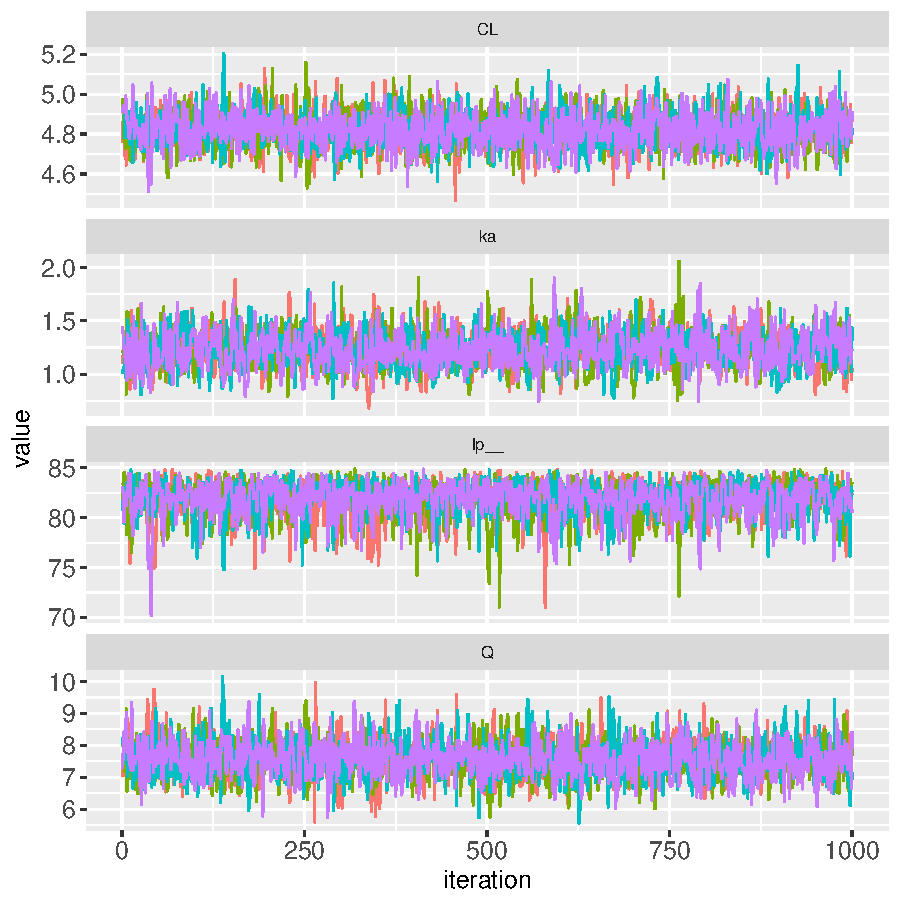
\includegraphics[width=0.6\linewidth]{../example-models/R/deliv/figure/TwoCptModel/TwoCptModelPlots001.pdf}
\caption{\label{fig:org0c822f0}
MCMC history plots for the parameters of a two compartment model with first order absorption (each color corresponds to a different chain)}
\end{figure}

\begin{figure}[htbp]
\centering
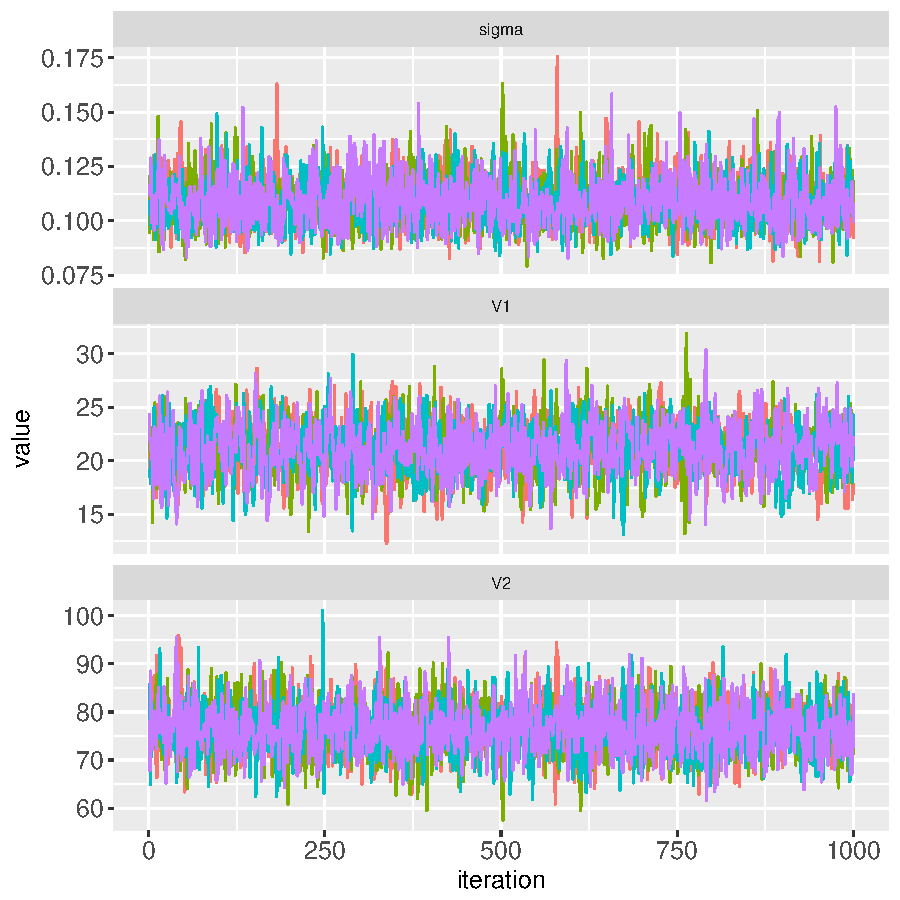
\includegraphics[width=0.6\linewidth]{../example-models/R/deliv/figure/TwoCptModel/TwoCptModelPlots002.pdf}
\caption{\label{fig:org514c5c2}
MCMC history plots for the parameters of a two compartment model with first order absorption (each color corresponds to a different chain)}
\end{figure}

\begin{figure}[htbp]
\centering
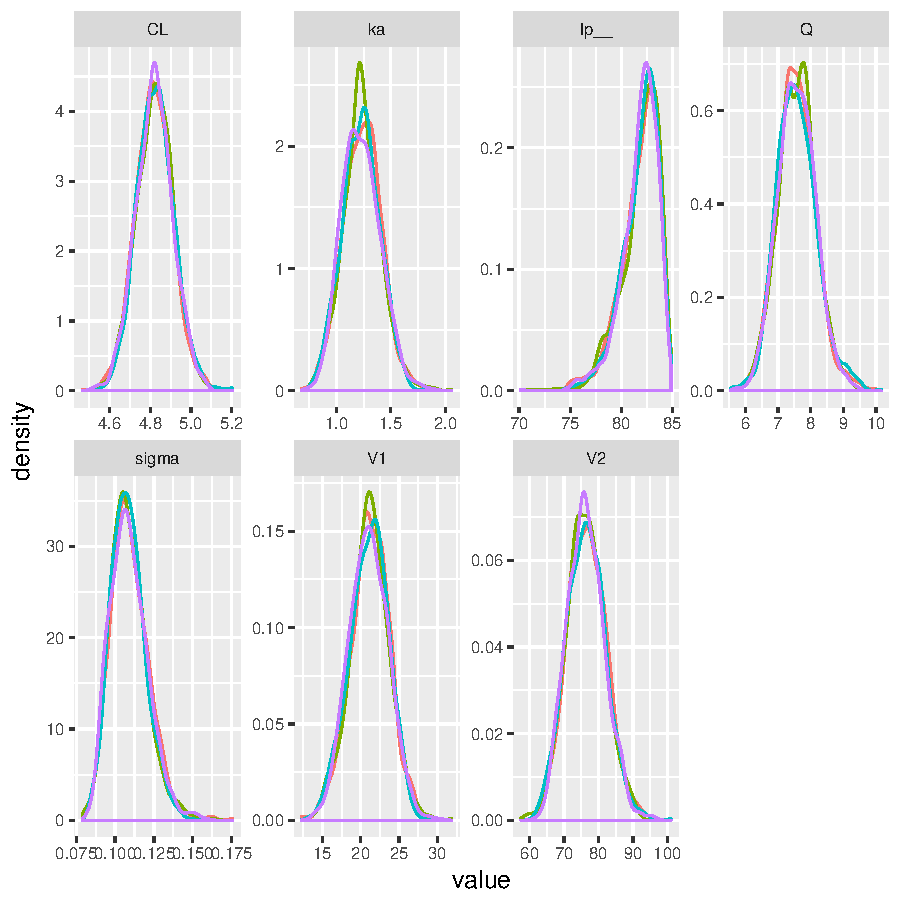
\includegraphics[width=0.6\linewidth]{../example-models/R/deliv/figure/TwoCptModel/TwoCptModelPlots003.pdf}
\caption{\label{fig:orgc22c74c}
Posterior Marginal Densities of the Model Parameters of a two compartment model with first order absorption (each color corresponds to a different chain)}
\end{figure}

\begin{figure}[htbp]
\centering
\includegraphics[width=0.5\linewidth]{../example-models/R/deliv/figure/TwoCptModel/TwoCptModelPlots006.pdf}
\caption{\label{fig:org85b2cc9}
Predicted (posterior median and 90\% credible intervals) and observed plasma drug concentrations of a two compartment model with first order absorption}
\end{figure}


\section{General Linear ODE Model Function}
\label{sec:org15b373c}
\index{General linear model}
\begin{minted}[breaklines=true,fontsize=\footnotesize,breakanywhere=true]{stan}
matrix linOdeModel(real[] time, real[] amt, real[] rate,
                   real[] ii, int[] evid, int[] cmt,
                   real[] addl, int[] ss,
                   matrix K, real[] biovar, real[] tlag)
\end{minted}
The Torsten function \texttt{linOdeModel} 
solves a (piecewise) linear ODEs model with coefficients
in form of a matrix \(K\)
%
\begin{equation}
y^\prime\left(t\right) = Ky\left(t\right)
\end{equation}
%
For example, for a two-compartment model with first order absorption, \(K\) would be

\begin{equation}
  K = \left[\begin{array}{ccc}
              -k_a & 0 & 0 \\
              k_a & -\left(k_{10} + k_{12}\right) & k_{21} \\
              0 & k_{12} & -k_{21}
            \end{array}\right]
\end{equation}
%
where \(k_{10}=CL/V_2\), \(k_{12}=Q/V_2\), and \(k_{21}=Q/V_3\).

\ \\
\begin{itemize}
\item \texttt{K} contains ODE coefficients and replaces \texttt{theta}. 
If \texttt{K} is constant across events, we can pass it as a matrix.
If it varies between events, \texttt{K} may be passed as an array of matrices.
The $i^\mathrm{th}$ element corresponds to the matrix in the interval \texttt{[time[i-1], time[i]]}.
The number of elements in the array is the number of events.
%
%In the case of constant rate,
%\texttt{K} is the same for all events or an array of constant rate
%matrices. The length of the array is
%the number of events and the \texttt{i} th element corresponds to the matrix at
%the interval \texttt{[time[i-1], time[i]]}.
%Note that \texttt{K} contains all the ODE parameters, so we no
%longer need \texttt{theta}.
\item See section \ref{org508cda2} regarding the model arguments \texttt{biovar}, and \texttt{tlag}.
\item The function returns a matrix with \texttt{nt} rows
and \texttt{n} columns, where \texttt{nt} is the number of time steps and
\texttt{n} is the size of the square matrix \texttt{K}.
\end{itemize}

\subsection{Example}
\label{sec:orge17e28a}
Using \texttt{linOdeModel}, the following example fits a two-compartment model
with first order absorption.

\begin{minted}[breaklines=true,fontsize=\footnotesize,breakanywhere=true]{stan}
// LinTwoCptModelExample.stan
// Run two compartment model using matrix exponential solution
// Heavily anotated to help new users

data{
  int<lower = 1> nt;  // number of events
  int<lower = 1> nObs;  // number of observations
  int<lower = 1> iObs[nObs];  // index of observation

  // NONMEM data
  int<lower = 1> cmt[nt];
  int evid[nt];
  int addl[nt];
  int ss[nt];
  real amt[nt];
  real time[nt];
  real rate[nt];
  real ii[nt];

  vector<lower = 0>[nObs] cObs;  // observed concentration (dependent variable)
}

transformed data{
  vector[nObs] logCObs = log(cObs);
  int nCmt = 3;
  real biovar[nCmt];
  real tlag[nCmt];

  for (i in 1:nCmt) {
    biovar[i] = 1;
    tlag[i] = 0;
  }
}

parameters{
  real<lower = 0> CL;
  real<lower = 0> Q;
  real<lower = 0> V1;
  real<lower = 0> V2;
  real<lower = 0> ka;
  real<lower = 0> sigma;

}

transformed parameters{
  matrix[3, 3] K;
  real k10 = CL / V1;
  real k12 = Q / V1;
  real k21 = Q / V2;
  vector<lower = 0>[nt] cHat;
  vector<lower = 0>[nObs] cHatObs;
  matrix<lower = 0>[nt, 3] x;

  K = rep_matrix(0, 3, 3);

  K[1, 1] = -ka;
  K[2, 1] = ka;
  K[2, 2] = -(k10 + k12);
  K[2, 3] = k21;
  K[3, 2] = k12;
  K[3, 3] = -k21;

  // linModel takes in the constant rate matrix, the object theta which
  // contains the biovariability fraction and the lag time of each compartment,
  // and the NONMEM data.
  x = linOdeModel(time, amt, rate, ii, evid, cmt, addl, ss,
                  K, biovar, tlag);
\end{minted}

\section{General ODE Model Function}
\label{sec:orgb60e784}
\index{General ODE Model}
\begin{minted}[breaklines=true,fontsize=\footnotesize,breakanywhere=true]{stan}
matrix generalOdeModel_rk45(ODE_system, int nCmt,
                            real[] time, real[] amt, real[] rate, real[] ii,
                            int[] evid, int[] cmt, real[] addl, int[] ss,
                            real[] theta, real[] biovar, real[] tlag,                      
                            real rel_tol, real abs_tol, int max_step);
\end{minted}
\begin{minted}[breaklines=true,fontsize=\footnotesize,breakanywhere=true]{stan}
matrix generalOdeModel_bdf(ODE_system, int nCmt,
                           real[] time, real[] amt, real[] rate, real[] ii,
                           int[] evid, int[] cmt, real[] addl, int[] ss,
                           real[] theta, real[] biovar, real[] tlag,                      
                           real rel_tol, real abs_tol, int max_step);
\end{minted}

The Torsten functions \texttt{generalOdeModel\_rk45} and
\texttt{generalOdeModel\_bdf} solve first-order ODEs with
user-specified first-order right-hand-side (RHS):
\begin{equation*}
y'(t) = f(t, y(t), \theta)
\end{equation*}
%
where $\theta$ corresponds to coefficients in the ODE, which can be passed using \texttt{theta}.
In the case where the \texttt{rate} vector \(r\) is non-zero, this equation becomes:
\begin{equation*}
y'(t) = f(t, y(t), \theta) + r
\end{equation*}

\begin{itemize}
\item User specifies \(f(t, y(t))\) by defining \texttt{ODE\_system}
inside the \texttt{functions} block (see section 19.2 of the
Stan reference manual for details and code below
for an example). The user does NOT include the rates in their
definition of \(f\). Torsten automatically corrects the derivatives when
the rates are non-zero.
\item \texttt{nCmt} is the number of compartments (or, equivalently, the
number of ODEs) in the model.
\item \texttt{rel\_tol}, \texttt{abs\_tol},
and \texttt{max\_step} are tuning parameters for the ODE integrator:
respectively the relative tolerance, the absolute tolerance, and the
maximum number of steps.
\item \texttt{generalOdeModel\_rk45} solves ODEs with Stan's Runge-Kutta
ODE solver function \texttt{integrate\_ode\_rk45}.
\item \texttt{generalOdeModel\_rk45} solves ODEs with Stan's Backward
Differentiation(BDF) ODE solver function \texttt{integrate\_ode\_bdf},
\item The values to use for the tuning parameters depends on the integrator and
the specifics of the ODE system. Reducing the tolerance parameters and
increasing the number of steps make for a more robust integrator but
can significantly slow down the algorithm. The following can be used
as a starting point: 
\begin{itemize}
\item \texttt{rel\_tol = 1e-6}
\item \texttt{abs\_tol = 1e-6}
\item \texttt{max\_step = 1e+6}
\end{itemize}
for rk45 integrator and
\begin{itemize}
\item \texttt{rel\_tol = 1e-10}
\item \texttt{abs\_tol = 1e-10}
\item \texttt{max\_step = 1e+8}
\end{itemize}
for the BDF integrator\footnote{These are the default tuning parameters for the integrators. Torsten functions do not have a default values for these parameters. The user must explicitly pass the tuning parameters to \texttt{generalOdeModel\_*()} .}.
Users should be prepared to adjust these
values. For additional information, see the Stan User's
Manual \cite{stan_team_2017}.
\item In the case of a multiple truncated infusion rate dosing regimen,
the bioavailability \texttt{biovar} and the amount \texttt{amt} cannot be passed as parameters.
\item See section \ref{org508cda2} regarding model arguments \texttt{theta},
\texttt{biovar}, and \texttt{tlag}.
\end{itemize}

\subsection{Example}
\label{sec:org6e723c6}
Using \texttt{generalOdeModel\_rk45}, the following example fits a two-compartment model
with first order absorption. User-defined function
\texttt{twoCptModelODE} describes the RHS of the ODEs.

\begin{minted}[breaklines=true,fontsize=\footnotesize,breakanywhere=true]{stan}
// GenTwoCptModelExample.stan
// Run two compartment model using numerical solution
// Heavily anotated to help new users

functions{

  // define ODE system for two compartmnt model
  real[] twoCptModelODE(real t,
                        real[] x,
                        real[] parms,
                        real[] rate,  // in this example, rate is treated as data
                        int[] dummy){

    // Parameters
    real CL = parms[1];
    real Q = parms[2];
    real V1 = parms[3];
    real V2 = parms[4];
    real ka = parms[5];

    // Re-parametrization
    real k10 = CL / V1;
    real k12 = Q / V1;
    real k21 = Q / V2;

    // Return object (derivative)
    real y[3];  // 1 element per compartment of
                // the model

    // PK component of the ODE system
    y[1] = -ka*x[1];
    y[2] = ka*x[1] - (k10 + k12)*x[2] + k21*x[3];
    y[3] = k12*x[2] - k21*x[3];

    return y;
  }

}
data{
  int<lower = 1> nt;  // number of events
  int<lower = 1> nObs;  // number of observations
  int<lower = 1> iObs[nObs];  // index of observation

  // NONMEM data
  int<lower = 1> cmt[nt];
  int evid[nt];
  int addl[nt];
  int ss[nt];
  real amt[nt];
  real time[nt];
  real rate[nt];
  real ii[nt];

  vector<lower = 0>[nObs] cObs;  // observed concentration (dependent variable)
}

transformed data{
  vector[nObs] logCObs = log(cObs);
  int nTheta = 5;   // number of parameters
  int nCmt = 3;   // number of compartments
  real biovar[nCmt];
  real tlag[nCmt];

  for (i in 1:nCmt) {
    biovar[i] = 1;
    tlag[i] = 0;
  }
}

parameters{
  real<lower = 0> CL;
  real<lower = 0> Q;
  real<lower = 0> V1;
  real<lower = 0> V2;
  real<lower = 0> ka;
  real<lower = 0> sigma;
}

transformed parameters{
  real theta[nTheta];
  vector<lower = 0>[nt] cHat;
  vector<lower = 0>[nObs] cHatObs;
  matrix<lower = 0>[nt, 3] x; 

  theta[1] = CL;
  theta[2] = Q;
  theta[3] = V1;
  theta[4] = V2;
  theta[5] = ka;

  // generalCptModel takes in the ODE system, the number of compartment 
  // (here we have a two compartment model with first order absorption, so
  // three compartments), the parameters matrix, the NONEM data, and the tuning
  // parameters (relative tolerance, absolute tolerance, and maximum number of steps)
  // of the ODE integrator. The user can choose between the bdf and the rk45 integrator.
  // Returns a matrix with the predicted amount in each compartment 
  // at each event.

//  x = generalOdeModel_bdf(twoCptModelODE, 3,
//                          time, amt, rate, ii, evid, cmt, addl, ss,
//                          theta, biovar, tlag,
//                          1e-8, 1e-8, 1e8);

   x = generalOdeModel_rk45(twoCptModelODE, 3,
                           time, amt, rate, ii, evid, cmt, addl, ss,
                           theta, biovar, tlag,
                           1e-6, 1e-6, 1e6);

  cHat = col(x, 2) ./ V1;

  for(i in 1:nObs){
    cHatObs[i] = cHat[iObs[i]];  // predictions for observed data records
  }
}
\end{minted}

\section{Mixed ODE Model Function}
\label{sec:orgd5d2c97}
\label{orgd6e813b}
\index{Mixed ODE Model}

\begin{minted}[breaklines=true,fontsize=\footnotesize,breakanywhere=true]{stan}
matrix mixOde1CptModel_rk45(reduced_ODE_system, int nOde,
                            real[] time, real[] amt, real[] rate,
                            real[] ii, int[] evid, int[] cmt, real[]
                            addl, int[] ss,
                            real[] theta, real[] biovar, real[] tlag,
                            real rel_tol, real abs_tol, real max_step)
\end{minted}
\begin{minted}[breaklines=true,fontsize=\footnotesize,breakanywhere=true]{stan}
matrix mixOde1CptModel_bdf(reduced_ODE_system, int nOde,
                            real[] time, real[] amt, real[] rate,
                            real[] ii, int[] evid, int[] cmt, real[]
                            addl, int[] ss,
                            real[] theta, real[] biovar, real[] tlag,
                            real rel_tol, real abs_tol, real max_step)
\end{minted}
\begin{minted}[breaklines=true,fontsize=\footnotesize,breakanywhere=true]{stan}
matrix mixOde2CptModel_rk45(reduced_ODE_system, int nOde,
                            real[] time, real[] amt, real[] rate,
                            real[] ii, int[] evid, int[] cmt, real[]
                            addl, int[] ss,
                            real[] theta, real[] biovar, real[] tlag,
                            real rel_tol, real abs_tol, real max_step)
\end{minted}
\begin{minted}[breaklines=true,fontsize=\footnotesize,breakanywhere=true]{stan}
matrix mixOde2CptModel_bdf(reduced_ODE_system, int nOde,
                            real[] time, real[] amt, real[] rate,
                            real[] ii, int[] evid, int[] cmt, real[]
                            addl, int[] ss,
                            real[] theta, real[] biovar, real[] tlag,
                            real rel_tol, real abs_tol, real max_step)
\end{minted}
When the ODE system consists of two subsystems in form of
\begin{align*}
  y_1^\prime &= f_1(t, y_1), \\
  y_2^\prime &= f_2(t, y_1, y_2),
\end{align*}
with \(y_1\), \(y_2\), \(f_1\), and \(f_2\) being vector-valued functions, and
\(y_1^\prime\) independent of \(y_2\), the solution can be
accelerated if \(y_1\) admits an analytical solution which can
be introduced into the ODE for \(y_2\) for numerical
integration. This structure arises in PK/PD
models, where \(y_1\) describes a forcing PK function and \(y_2\) the PD
effects. In the example of a Friberg-Karlsson
semi-mechanistic model \cite{friberg_mechanistic_2003} (see below), we observe an average speedup of
\(\sim 47 \pm 18 \%\) when using the mix solver in lieu of the numerical
integrator \cite{margossian_mixed_2017}. Torsten supports the mixed solver for
cases where \(y_1\) solves the ODEs for a One or Two Compartment model
with a first-order absorption.

The \texttt{reduced\_ODE\_system} specifies the system we
numerically solve, \(y_2\) in the above discussion, also called the
\emph{reduced system}. \texttt{nOde} is the number of equations in
the \underline{reduced} system. The function that defines a reduced
system has an almost identical signature to that used for a full
system, but takes one additional argument: \(y_1\), the PK states,
i.e. solution to the PK ODEs.
\begin{minted}[breaklines=true,fontsize=\footnotesize,breakanywhere=true]{stan}
real[] reducedODE(real t,       // time
                  real[] y,     // reduced state
                  real[] y1,    // PK states
                  real[] theta, // parameters
                  real[] x_r,   // data (real)
                  int[] x_int)  // data (integer)
\end{minted}

The four functions of mixed solver correspond to all the permutations Torsten
provides when using a forcing One or Two Compartment function, and the
Runge-Kutta 4th/5th order (\texttt{rk45}) or Backward Differentiation (\texttt{bdf})
integration scheme. The mixed ODE functions can be used to compute the
steady state solutions supported by the general ODE model functions.

Restrictions regarding which arguments may be passed as parameters for
general ODE solvers also apply to
mixed solvers.

\section{Example}
\label{sec:orgba37f3d}
\index{Friberg-Karlsson Model}

A Friberg-Karlsson Semi-Mechanistic model \cite{friberg_mechanistic_2003} couples
a PK model with a PD
effect. In the current example, we use the two compartment model in section \ref{orge037615} for
the PK model.

Neutropenia is observed in patients receiving an ME-2 drug. Our goal
is to model the relation between neutrophil counts and drug
exposure. Using a feedback mechanism, the body maintains the number of
neutrophils at a baseline value (Figure \ref{fig:org9b72a2b}). While in the
patient's blood, the drug impedes the production of neutrophils. As a
result, the neutrophil count goes down. After the drug clears out, the
feedback mechanism kicks in and brings the neutrophil count back to
baseline.

\begin{align}
  \log(ANC_i) \sim& N(\log(Circ), \sigma^2_{ANC})  \\
  Circ =& f_{FK}(MTT, Circ_{0}, \alpha, \gamma, c)  \\
  (MTT, Circ_{0}, \alpha, \gamma, ktr) =& (125, 5.0, 3 \times 10^{-4}, 0.17) \\
  \sigma^2_{ANC} =& 0.001
\end{align}
where \(c\) is the drug concentration in the blood we get from the Two
Compartment model, and \(Circ\) is obtained by solving the following
system of nonlinear ODEs:
\begin{subequations}
  \begin{align}
   y_\mathrm{prol}' &= k_\mathrm{prol} y_\mathrm{prol} (1 - E_\mathrm{drug})\left(\frac{Circ_0}{y_\mathrm{circ}}\right)^\gamma - k_\mathrm{tr}y_\mathrm{prol} \\
   y_\mathrm{trans1}' &= k_\mathrm{tr} y_\mathrm{prol} - k_\mathrm{tr} y_\mathrm{trans1} \\
   y_\mathrm{trans2}' &= k_\mathrm{tr} y_\mathrm{trans1} - k_\mathrm{tr} y_\mathrm{trans2}  \\
   y_\mathrm{trans3}' &= k_\mathrm{tr} y_\mathrm{trans2} - k_\mathrm{tr} y_\mathrm{trans3}  \\
   y_\mathrm{circ}' &= k_\mathrm{tr} y_\mathrm{trans3} - k_\mathrm{tr} y_\mathrm{circ}
   \end{align}
   \label{eq:FK}
\end{subequations}
where \(E_{drug}  = \alpha c\).

The ODEs specifying the Two Compartment Model
(Equation \eqref{eq:twocpt}) do not depend on the PD ODEs
(Equation \eqref{eq:FK}) and can be solved analytically
using Torsten's \mintinline[breaklines=true,fontsize=\footnotesize,breakanywhere=true]{stan}{PKModelTwoCpt} function. We
therefore specify our model using a mixed solver function. We do not
expect our system to be stiff and use the Runge-Kutta 4th/5th order
integrator.

\begin{figure}[htbp]
\centering
\includegraphics[width=0.8\textwidth]{./graphics/neutrophilModel.jpg}
\caption{\label{fig:org9b72a2b}
Friberg-Karlsson semi-mechanistic Model.}
\end{figure}

\begin{minted}[breaklines=true,fontsize=\footnotesize,breakanywhere=true]{stan}
functions{
  real[] FK_ODE(real t,
                real[] y,
                real[] y_pk,
                real[] theta,
                real[] rdummy,
                int[] idummy){
    /* PK variables */
    real VC = theta[3];

    /* PD variable */
    real mtt      = theta[6];
    real circ0    = theta[7];
    real alpha    = theta[8];
    real gamma    = theta[9];
    real ktr      = 4.0 / mtt;
    real prol     = y[1] + circ0;
    real transit1 = y[2] + circ0;
    real transit2 = y[3] + circ0;
    real transit3 = y[4] + circ0;
    real circ     = fmax(machine_precision(), y[5] + circ0);
    real conc     = y_pk[2] / VC;
    real EDrug    = alpha * conc;

    real dydt[5];

    dydt[1] = ktr * prol * ((1 - EDrug) * ((circ0 / circ)^gamma) - 1);
    dydt[2] = ktr * (prol - transit1);
    dydt[3] = ktr * (transit1 - transit2);
    dydt[4] = ktr * (transit2 - transit3);
    dydt[5] = ktr * (transit3 - circ);

    return dydt;
  }
}

data{
  int<lower = 1> nt;
  int<lower = 1> nObsPK;
  int<lower = 1> nObsPD;
  int<lower = 1> iObsPK[nObsPK];
  int<lower = 1> iObsPD[nObsPD];
  real<lower = 0> amt[nt];
  int<lower = 1> cmt[nt];
  int<lower = 0> evid[nt];
  real<lower = 0> time[nt];
  real<lower = 0> ii[nt];
  int<lower = 0> addl[nt];
  int<lower = 0> ss[nt];
  real rate[nt];
  vector<lower = 0>[nObsPK] cObs;
  vector<lower = 0>[nObsPD] neutObs;

  real<lower = 0> circ0Prior;
  real<lower = 0> circ0PriorCV;
  real<lower = 0> mttPrior;
  real<lower = 0> mttPriorCV;
  real<lower = 0> gammaPrior;
  real<lower = 0> gammaPriorCV;
  real<lower = 0> alphaPrior;
  real<lower = 0> alphaPriorCV;
}

transformed data{
  int nOde = 5;
  vector[nObsPK] logCObs;
  vector[nObsPD] logNeutObs;
//  int idummy[0];
//  real rdummy[0];

  int nTheta;
  int nIIV;

  int n;                        /* ODE dimension */
  real rtol;
  real atol;
  int max_step;

  n = 8;
  rtol = 1e-8;
  atol = 1e-8;
  max_step = 100000;

  logCObs = log(cObs);
  logNeutObs = log(neutObs);

  nIIV = 7; // parameters with IIV
  nTheta = 9; // number of parameters
}

parameters{

  real<lower = 0> CL;
  real<lower = 0> Q;
  real<lower = 0> VC;
  real<lower = 0> VP;
  real<lower = 0> ka;
  real<lower = 0> mtt;
  real<lower = 0> circ0;
  real<lower = 0> alpha;
  real<lower = 0> gamma;
  real<lower = 0> sigma;
  real<lower = 0> sigmaNeut;

  // IIV parameters
  cholesky_factor_corr[nIIV] L;
  vector<lower = 0>[nIIV] omega;
}

transformed parameters{
  vector[nt] cHat;
  vector<lower = 0>[nObsPK] cHatObs;
  vector[nt] neutHat;
  vector<lower = 0>[nObsPD] neutHatObs;
  real<lower = 0> theta[nTheta];
  matrix[nt, nOde + 3] x;
  real biovar[nTheta];
  real tlag[nTheta];

  for (i in 1:nTheta) {
    biovar[i] = 1.0;
    tlag[i] = 0.0;
  }

  theta[1] = CL;
  theta[2] = Q;
  theta[3] = VC;
  theta[4] = VP;
  theta[5] = ka;
  theta[6] = mtt;
  theta[7] = circ0;
  theta[8] = alpha;
  theta[9] = gamma;

  x = mixOde2CptModel_rk45(FK_ODE, nOde, time, amt, rate, ii, evid, cmt, addl, ss, theta, biovar, tlag, rtol, atol, max_step);

  cHat = col(x, 2) / VC;
  neutHat = col(x, 8) + circ0;

  for(i in 1:nObsPK) cHatObs[i]    = cHat[iObsPK[i]];
  for(i in 1:nObsPD) neutHatObs[i] = neutHat[iObsPD[i]];

}

model {

  // Priors
  CL    ~ normal(0, 20);
  Q     ~ normal(0, 20);
  VC    ~ normal(0, 100);
  VP    ~ normal(0, 1000);
  ka    ~ normal(0, 5);
  sigma ~ cauchy(0, 1);

  mtt       ~ lognormal(log(mttPrior), mttPriorCV);
  circ0     ~ lognormal(log(circ0Prior), circ0PriorCV);
  alpha     ~ lognormal(log(alphaPrior), alphaPriorCV);
  gamma     ~ lognormal(log(gammaPrior), gammaPriorCV);
  sigmaNeut ~ cauchy(0, 1);

  // Parameters for Matt's trick
  L ~ lkj_corr_cholesky(1);
  omega ~ cauchy(0, 1);

  // observed data likelihood
  logCObs ~ normal(log(cObs), sigma);
  logNeutObs ~ normal(log(neutObs), sigmaNeut);
}
\end{minted}

\section{Univariate integral}
\label{sec:org8b99740}
\index{univariate integral}
\begin{minted}[breaklines=true,fontsize=\footnotesize,breakanywhere=true]{stan}
real univariate_integral_rk45(f, t0, t1, theta, x_r, x_i)
\end{minted}
\begin{minted}[breaklines=true,fontsize=\footnotesize,breakanywhere=true]{stan}
real univariate_integral_bdf(f, t0, t1, theta, x_r, x_i)
\end{minted}
Based on the ODE solver capability in Stan, Torsten provides functions
calculating the integral of a univariate function. The integrand function \(f\) must follow the signature
\begin{minted}[breaklines=true,fontsize=\footnotesize,breakanywhere=true]{stan}
  real f(real t, real[] theta, real[] x_r, int[] x_i) {
    /* ... */
}
\end{minted}

\subsection{Example}
\label{sec:org6809fc1}
This example shows how to use \texttt{univariate\_integral\_rk45} to calculate the
integral of a quadratic function.
\begin{minted}[breaklines=true,fontsize=\footnotesize,breakanywhere=true]{stan}
functions {
  real fun_ord2(real t, real[] theta, real[] x_r, int[] x_i) {
    real a = 2.3;
    real b = 2.0;
    real c = 1.5;
    real res;
    res = a + b * t + c * t * t;
    return res;
  }
}
data {
  real t0;
  real t1;
  real dtheta[2];
  real x_r[0];
  int x_i[0];
}
transformed data {
  real univar_integral;
  univar_integral = univariate_integral_rk45(func, t0, t1, dtheta, 
                          x_r, x_i);
}
/* ... */
\end{minted}


\section{Piecewise linear interpolation}
\label{sec:org8d847b4}
\index{linear interpolation}
\begin{minted}[breaklines=true,fontsize=\footnotesize,breakanywhere=true]{stan}
real linear_interpolation(real xout, real[] x, real[] y)
\end{minted}
\begin{minted}[breaklines=true,fontsize=\footnotesize,breakanywhere=true]{stan}
real[] linear_interpolation(real[] xout, real[] x, real[] y)
\end{minted}
Torsten also provides a \texttt{linear\_interpolation} function for piecewise linear interpolation over a
set of x, y pairs. It returns the values of a piecewise linear
function at specified values \texttt{xout} of the first function argument. The
function is specified in terms of a set of x, y
pairs. Specifically, \texttt{linear\_interpolation} implements the following function
\begin{align*}
  y_{\text{out}} = \left\{\begin{array}{ll}
                 y_1, & x_{\text{out}} < x_1 \\
                 y_i + \frac{y_{i+1} - y_i}{x_{i+1} - x_i}
                 \left(x_{\text{out}} - x_i\right), & x_{\text{out}} \in [x_i, x_{i+1}) \\
                 y_n, & x_{\text{out}} \ge x_n 
                          \end{array}\right.
\end{align*}
\begin{itemize}
\item The x values must be in increasing order, i.e. \(x_i < x_{i+1}\).
\item All three arguments may be data or parameters.
\end{itemize}
\subsection{Example}
\label{sec:orgf03d923}
This example illustrates how to use \texttt{linear\_intepolationi}
to fit a piecewise linear function to a data set consisting
of \((x, y)\) pairs.
\begin{minted}[breaklines=true,fontsize=\footnotesize,breakanywhere=true]{stan}
data{
  int nObs;
  real xObs[nObs];
  real yObs[nObs];
  int nx;
  int nPred;
  real xPred[nPred];
}

transformed data{
  real xmin = min(xObs);
  real xmax = max(xObs);
}

parameters{
  real y[nx];
  real<lower = 0> sigma;
  simplex[nx - 1] xSimplex;
}

transformed parameters{
  real yHat[nObs];
  real x[nx];

  x[1] = xmin;
  x[nx] = xmax;
  for(i in 2:(nx-1))
    x[i] = x[i-1] + xSimplex[i-1] * (xmax - xmin);

  yHat = linear_interpolation(xObs, x, y);
}

model{
  xSimplex ~ dirichlet(rep_vector(1, nx - 1));
  y ~ normal(0, 25);
  yObs ~ normal(yHat, sigma);
}

generated quantities{
  real yHatPred[nPred];
  real yPred[nPred];

  yHatPred = linear_interpolation(xPred, x, y);
  for(i in 1:nPred)
    yPred[i] = normal_rng(yHatPred[i], sigma);
}
\end{minted}

\chapter{Additional examples}
\label{sec:org2d27c6c}
\section{Effect Compartment Population Model}
\label{sec:org41e1a30}
Here we expand the example in \ref{orge037615} to a population model fitted to the
combined data from phase I and phase IIa studies. The
parameters exhibit inter-individual variations (IIV), due to
both random effects and to the patients' body weight,
treated as a covariate and denoted \(bw\).
\subsection{Population Model for Plasma Drug Concentration \(c\)}
\label{sec:orgf446826}
\begin{gather*}
  \log\left(c_{ij}\right) \sim N\left(\log\left(\widehat{c}_{ij}\right),\sigma^2\right), \\
  \widehat{c}_{ij} = f_{2cpt}\left(t_{ij},D_j,\tau_j,CL_j,Q_j,V_{1j},V_{2j},k_{aj}\right), \\
  \log\left(CL_j,Q_j,V_{ssj},k_{aj}\right) \sim N\left(\log\left(\widehat{CL}\left(\frac{bw_j}{70}\right)^{0.75},\widehat{Q}\left(\frac{bw_j}{70}\right)^{0.75}, \widehat{V}_{ss}\left(\frac{bw_j}{70}\right),\widehat{k}_a\right),\Omega\right), \\
  V_{1j} = f_{V_1}V_{ssj}, \\
  V_{2j} = \left(1 - f_{V_1}\right)V_{ssj}, \\
  \left(\widehat{CL},\widehat{Q},\widehat{V}_{ss},\widehat{k}_a, f_{V_1}\right) = \left(10\ {\rm L/h},15\  {\rm L/h},140\  {\rm L},2\ {\rm h^{-1}}, 0.25 \right), \\
  \Omega = \left(\begin{array}{cccc} 0.25^2 & 0 & 0 & 0 \\ 0 & 0.25^2 & 0 & 0 \\
                    0 & 0 & 0.25^2 & 0 \\ 0 & 0 & 0 & 0.25^2  \end{array}\right), \\
  \sigma = 0.1
\end{gather*}

Furthermore we add a fourth compartment in which we measure
a PD effect(Figure \ref{fig:org8cfda29}).

\begin{figure}[htbp]
\centering
\includegraphics[width=0.5\textwidth]{./graphics/effCptModel.png}
\caption{\label{fig:org8cfda29}
Effect Compartment Model}
\end{figure}

\subsection{Effect Compartment Model for PD response \(R\).}
\label{sec:orgd4e5fa2}
\begin{gather*}
R_{ij} \sim N\left(\widehat{R}_{ij},\sigma_{R}^2\right), \\
\widehat{R}_{ij} = \frac{E_{max}c_{eij}}{EC_{50j} + c_{eij}}, \\
c_{e\cdot j}^\prime = k_{e0j}\left(c_{\cdot j} - c_{e\cdot j}\right), \\
\log\left(EC_{50j}, k_{e0j}\right) \sim N\left(\log\left(\widehat{EC}_{50}, \widehat{k}_{e0}\right),\Omega_R\right), \\
\left(E_{max}, \widehat{EC}_{50},\widehat{k}_{e0}\right) = \left(100, 100.7, 1\right), \\
\Omega_R = \left(\begin{array}{cc} 0.2^2 & 0 \\ 0 & 0.25^2  \end{array}\right), \ \ \ \sigma_R = 10.
\end{gather*}

The PK and the PD data are simulated using the following
treatment.
\begin{itemize}
\item Phase I study
\begin{itemize}
\item Single dose and multiple doses
\item Parallel dose escalation design
\item 25 subjects per dose
\item Single doses: 1.25, 5, 10, 20, and 40 mg
\item PK: plasma concentration of parent drug (\(c\))
\item PD response: Emax function of effect compartment concentration (\(R\))
\item PK and PD measured at 0.083, 0.167, 0.25, 0.5, 0.75, 1, 2, 3, 4, 6, 8, 12, 18, and 24 hours
\end{itemize}
\item Phase IIa trial in patients
\begin{itemize}
\item 100 subjects
\item Multiple doses: 20 mg
\item sparse PK and PD data (3-6 samples per patient)
\end{itemize}
\end{itemize}

The model is simultaneously fitted to the PK and the PD
data. For this effect compartment model, we construct a
constant rate matrix and use \texttt{linOdeModel}. Correct use of
Torsten requires the user pass the entire event history
(observation and dosing events) for an individual to the
function. Thus the Stan model shows the call to \texttt{linOdeModel}
within a loop over the individual subjects rather than over
the individual observations.

\begin{minted}[breaklines=true,fontsize=\footnotesize,breakanywhere=true]{stan}
transformed parameters{
  vector<lower = 0>[nRandom] thetaHat;
  cov_matrix[nRandom] Omega;
  real<lower = 0> CL[nSubjects];
  real<lower = 0> Q[nSubjects];
  real<lower = 0> V1[nSubjects];
  real<lower = 0> V2[nSubjects];
  real<lower = 0> ka[nSubjects];
  real<lower = 0> ke0[nSubjects];
  real<lower = 0> EC50[nSubjects];
  matrix[nCmt, nCmt] K;
  real k10;
  real k12;
  real k21;
  vector<lower = 0>[nt] cHat;
  vector<lower = 0>[nObs] cHatObs;
  vector<lower = 0>[nt] respHat;
  vector<lower = 0>[nObs] respHatObs;
  vector<lower = 0>[nt] ceHat;
  matrix[nt, nCmt] x;

  thetaHat[1] = CLHat;
  thetaHat[2] = QHat;
  thetaHat[3] = V1Hat;
  thetaHat[4] = V2Hat;
  thetaHat[5] = kaHat;

  Omega = quad_form_diag(rho, omega); ## diag_matrix(omega) * rho * diag_matrix(omega)

  for(j in 1:nSubjects){
    CL[j] = exp(logtheta[j, 1]) * (weight[j] / 70)^0.75;
    Q[j] = exp(logtheta[j, 2]) * (weight[j] / 70)^0.75;
    V1[j] = exp(logtheta[j, 3]) * weight[j] / 70;
    V2[j] = exp(logtheta[j, 4]) * weight[j] / 70;
    ka[j] = exp(logtheta[j, 5]);
    ke0[j] = exp(logKe0[j]);
    EC50[j] = exp(logEC50[j]);

    k10 = CL[j] / V1[j];
    k12 = Q[j] / V1[j];
    k21 = Q[j] / V2[j];

    K = rep_matrix(0, nCmt, nCmt);

    K[1, 1] = -ka[j];
    K[2, 1] = ka[j];
    K[2, 2] = -(k10 + k12);
    K[2, 3] = k21;
    K[3, 2] = k12;
    K[3, 3] = -k21;
    K[4, 2] = ke0[j];
    K[4, 4] = -ke0[j];

    x[start[j]:end[j],] = linOdeModel(time[start[j]:end[j]],
                                      amt[start[j]:end[j]],
                                      rate[start[j]:end[j]],
                                      ii[start[j]:end[j]],
                                      evid[start[j]:end[j]],
                                      cmt[start[j]:end[j]],
                                      addl[start[j]:end[j]],
                                      ss[start[j]:end[j]],
                                      K, biovar, tlag);

    cHat[start[j]:end[j]] = 1000 * x[start[j]:end[j], 2] ./ V1[j];
    ceHat[start[j]:end[j]] = 1000 * x[start[j]:end[j], 4] ./ V1[j];
    respHat[start[j]:end[j]] = 100 * ceHat[start[j]:end[j]] ./ 
       (EC50[j] + ceHat[start[j]:end[j]]);
  }

  cHatObs = cHat[iObs];
  respHatObs = respHat[iObs];

}
\end{minted}

\subsection{Results}
\label{sec:org6596fdb}
We use the same diagnosis tools as for the
previous examples. The MCMC history plots (Figure \ref{effCptModelMCMC}) suggest the 4 chains have converged to common
distributions. We note some minor auto-correlations for \(lp\_\) (the
log posterior) and for IIV parameters: specifically \(\Omega_{ke_0}\)
and \(\rho\). The correlation matrix \(\rho\) does not explicitly appear
in the model, but it is used to construct \(\Omega\), which parametrizes
the PK IIV. 
The fits to the plasma concentration
(Figure \ref{effCptModelPredictionsPK}) are in close agreement with
the data, notably for the sparse data case (phase IIa study). The fits
to the PD data (Figure \ref{effCptModelPredictionsPD}) look good,
though the data is more noisy. The model reflects the noise by
producing larger credible intervals. The estimated values of the
parameters are consistent with the values used to simulate the data
(Table \ref{tab:org9ac148e}) and Figure \ref{effCptModelDens}).

\begin{table}[htbp]
\caption{\label{tab:org9ac148e}
Summary of the MCMC simulations of the marginal posterior distributions of the model parameters for the effect compartment model example.}
\centering
\footnotesize
\begin{tabular}{r r r r r r r r r r r}
 & mean & se\_mean & sd & 2.5\% & 25\% & 50\% & 75\% & 97.5\% & n\_eff & Rhat\\
\hline
lp\_\_ & -201.282 & 10.073 & 84.189 & -333.764 & -259.017 & -213.416 & -154.381 & 8.549 & 69.850 & 1.044\\
CLHat & 10.095 & 0.003 & 0.201 & 9.712 & 9.958 & 10.096 & 10.231 & 10.483 & 4000.000 & 0.999\\
QHat & 14.867 & 0.014 & 0.357 & 14.182 & 14.620 & 14.862 & 15.106 & 15.563 & 678.208 & 1.007\\
V1Hat & 34.188 & 0.067 & 1.089 & 31.940 & 33.494 & 34.214 & 34.918 & 36.251 & 267.748 & 1.016\\
V2Hat & 103.562 & 0.076 & 2.925 & 98.031 & 101.600 & 103.454 & 105.472 & 109.583 & 1488.296 & 1.001\\
kaHat & 1.930 & 0.004 & 0.077 & 1.771 & 1.880 & 1.933 & 1.982 & 2.076 & 334.888 & 1.014\\
ke0Hat & 1.050 & 0.001 & 0.044 & 0.967 & 1.020 & 1.051 & 1.078 & 1.137 & 1164.741 & 1.000\\
EC50Hat & 104.337 & 0.040 & 2.100 & 100.169 & 102.909 & 104.345 & 105.768 & 108.351 & 2744.041 & 1.000\\
sigma & 0.099 & 0.000 & 0.002 & 0.095 & 0.097 & 0.099 & 0.100 & 0.103 & 1906.342 & 1.002\\
sigmaResp & 10.156 & 0.003 & 0.197 & 9.779 & 10.023 & 10.154 & 10.286 & 10.552 & 4000.000 & 1.000\\
omega[1] & 0.270 & 0.000 & 0.016 & 0.241 & 0.259 & 0.269 & 0.280 & 0.302 & 4000.000 & 1.001\\
omega[2] & 0.231 & 0.001 & 0.021 & 0.192 & 0.217 & 0.230 & 0.245 & 0.275 & 531.512 & 1.006\\
omega[3] & 0.219 & 0.002 & 0.031 & 0.158 & 0.199 & 0.218 & 0.238 & 0.281 & 158.198 & 1.017\\
omega[4] & 0.267 & 0.001 & 0.026 & 0.218 & 0.249 & 0.266 & 0.284 & 0.319 & 684.870 & 1.001\\
omega[5] & 0.285 & 0.002 & 0.037 & 0.214 & 0.259 & 0.284 & 0.309 & 0.361 & 284.545 & 1.009\\
omegaKe0 & 0.271 & 0.003 & 0.047 & 0.183 & 0.239 & 0.271 & 0.303 & 0.363 & 217.350 & 1.007\\
omegaEC50 & 0.213 & 0.001 & 0.021 & 0.174 & 0.199 & 0.213 & 0.227 & 0.255 & 1190.193 & 1.000\\
rho[1,2] & 0.194 & 0.003 & 0.100 & -0.011 & 0.127 & 0.195 & 0.265 & 0.379 & 1000.772 & 1.004\\
rho[1,3] & -0.157 & 0.005 & 0.126 & -0.395 & -0.243 & -0.157 & -0.072 & 0.088 & 677.709 & 1.001\\
rho[2,3] & 0.079 & 0.012 & 0.155 & -0.227 & -0.024 & 0.082 & 0.181 & 0.384 & 180.306 & 1.021\\
rho[1,4] & -0.107 & 0.003 & 0.112 & -0.319 & -0.183 & -0.110 & -0.032 & 0.118 & 1081.932 & 1.002\\
rho[2,4] & 0.194 & 0.005 & 0.126 & -0.062 & 0.110 & 0.199 & 0.282 & 0.428 & 623.035 & 1.007\\
rho[3,4] & 0.796 & 0.008 & 0.094 & 0.592 & 0.737 & 0.808 & 0.867 & 0.940 & 152.112 & 1.033\\
rho[1,5] & 0.023 & 0.006 & 0.135 & -0.232 & -0.068 & 0.024 & 0.115 & 0.285 & 564.687 & 1.003\\
rho[2,5] & 0.119 & 0.011 & 0.160 & -0.188 & 0.008 & 0.118 & 0.224 & 0.438 & 226.174 & 1.014\\
rho[3,5] & -0.246 & 0.018 & 0.202 & -0.663 & -0.382 & -0.237 & -0.105 & 0.133 & 119.465 & 1.021\\
rho[4,5] & -0.288 & 0.009 & 0.155 & -0.576 & -0.396 & -0.291 & -0.183 & 0.014 & 275.549 & 1.009\\
\end{tabular}
\end{table}

\begin{figure}[!htb]
  \includegraphics[width=3.0in,trim=0in 0in 0 0in]{graphics/effCptModelTorsten_0.82/effCptPlots001.pdf}
  \includegraphics[width=3.0in,trim=0in 0in 0 0in]{graphics/effCptModelTorsten_0.82/effCptPlots002.pdf}
  \includegraphics[width=3.0in,trim=0in 0in 0 0in]{graphics/effCptModelTorsten_0.82/effCptPlots003.pdf}
  \includegraphics[width=3.0in,trim=0in 0in 0 0in]{graphics/effCptModelTorsten_0.82/effCptPlots004.pdf}
  \includegraphics[width=3.0in,trim=0in 0in 0 0in]{graphics/effCptModelTorsten_0.82/effCptPlots005.pdf}
  \caption{{MCMC history plots for the parameters of an Effect Compartment Model (each color corresponds to a different chain) for example 2}}
  \label{effCptModelMCMC}
\end{figure}

\begin{figure}[!htb]
  \includegraphics[width=3.0in,trim=0in 0in 0 0in]{graphics/effCptModelTorsten_0.82/effCptPlots006.pdf}
  \includegraphics[width=3.0in,trim=0in 0in 0 0in]{graphics/effCptModelTorsten_0.82/effCptPlots007.pdf}
  \caption{{Posterior Marginal Densities of the Model Parameters of an Effect Compartment Model (each color corresponds to a different chain) for example 2}}
  \label{effCptModelDens}
\end{figure}

\begin{figure}[!htb]
  \includegraphics[width=1.5in,trim=0in 0in 0 0in]{graphics/effCptModelTorsten_0.82/effCptPlots011.pdf}
  \includegraphics[width=1.5in,trim=0in 0in 0 0in]{graphics/effCptModelTorsten_0.82/effCptPlots012.pdf}
  \includegraphics[width=1.5in,trim=0in 0in 0 0in]{graphics/effCptModelTorsten_0.82/effCptPlots013.pdf}
  \includegraphics[width=1.5in,trim=0in 0in 0 0in]{graphics/effCptModelTorsten_0.82/effCptPlots014.pdf}
  \includegraphics[width=1.5in,trim=0in 0in 0 0in]{graphics/effCptModelTorsten_0.82/effCptPlots019.pdf}
  \includegraphics[width=1.5in,trim=0in 0in 0 0in]{graphics/effCptModelTorsten_0.82/effCptPlots020.pdf}
  \includegraphics[width=1.5in,trim=0in 0in 0 0in]{graphics/effCptModelTorsten_0.82/effCptPlots021.pdf}
  \includegraphics[width=1.5in,trim=0in 0in 0 0in]{graphics/effCptModelTorsten_0.82/effCptPlots022.pdf}
  \caption{{Predicted (posterior median and 90 \% credible intervals) and observed plasma drug concentrations for example 2 for an Effect Compartment Model}}
  \label{effCptModelPredictionsPK}
\end{figure}

\begin{figure}[!htb]
\includegraphics[width=1.5in,trim=0in 0in 0 0in]{graphics/effCptModelTorsten_0.82/effCptPlots023.pdf}
\includegraphics[width=1.5in,trim=0in 0in 0 0in]{graphics/effCptModelTorsten_0.82/effCptPlots024.pdf}
\includegraphics[width=1.5in,trim=0in 0in 0 0in]{graphics/effCptModelTorsten_0.82/effCptPlots025.pdf}
\includegraphics[width=1.5in,trim=0in 0in 0 0in]{graphics/effCptModelTorsten_0.82/effCptPlots026.pdf}
\includegraphics[width=1.5in,trim=0in 0in 0 0in]{graphics/effCptModelTorsten_0.82/effCptPlots027.pdf}
\includegraphics[width=1.5in,trim=0in 0in 0 0in]{graphics/effCptModelTorsten_0.82/effCptPlots028.pdf}
\includegraphics[width=1.5in,trim=0in 0in 0 0in]{graphics/effCptModelTorsten_0.82/effCptPlots029.pdf}
\includegraphics[width=1.5in,trim=0in 0in 0 0in]{graphics/effCptModelTorsten_0.82/effCptPlots030.pdf}
\caption{{Predicted (posterior median and 90 \% credible intervals) and observed PD Response for example 2}}
\label{effCptModelPredictionsPD}
\end{figure}

\section{Friberg-Karlsson Semi-Mechanistic Population Model}
\label{sec:org84102b2}
We now return to the example in Section \ref{orgd6e813b} and extend
it to a population model. While we recommend using the mixed
solver, for completeness we show how to specify the model
with the \texttt{generalOdeModel} function. We leave it
as an exercise to the reader to rewrite the model with
\texttt{mixOde2CptModel}. 

\subsection{Friberg-Karlsson Population Model for drug-induced myelosuppression (\(ANC\))}
\label{sec:org3648344}
\begin{gather*}
\log(ANC_{ij}) \sim N(Circ_{ij}, \sigma^2_{ANC}), \\
\log\left(MTT_j, Circ_{0j}, \alpha_j\right) \sim N\left(\log\left(\widehat{MTT}, \widehat{Circ_0}, \widehat{\alpha}\right), \Omega_{ANC}\right), \\
\left(\widehat{MTT}, \widehat{Circ}_0,\widehat{\alpha}, \gamma \right) = \left(125, 5, 2, 0.17\right), \\
\Omega_{ANC} = \left(\begin{array}{ccc} 0.2^2 & 0 & 0 \\ 0 & 0.35^2 & 0 \\ 0 & 0 & 0.2^2 \end{array}\right), \\
\sigma_{ANC} = 0.1, \\
\Omega_{PK} = \left(\begin{array}{ccccc} 0.25^2 & 0 &a 0 & 0 & 0 \\ 0 & 0.4^2 & 0 & 0 & 0 \\
0 & 0 & 0.25^2 & 0 & 0 \\ 0 & 0 & 0 & 0.4^2 & 0 \\ 0 & 0 & 0 & 0 & 0.25^2  \end{array}\right)
\end{gather*}
The PK and the PD data are simulated using the following treatment.
\begin{itemize}
\item Phase IIa trial in patients
\begin{itemize}
\item Multiple doses: 80,000 mg
\item Parallel dose escalation design
\item 15 subjects
\item PK: plasma concentration of parent drug (\(c\))
\item PD response: Neutrophil count (\(ANC\))
\item PK measured at 0.083, 0.167, 0.25, 0.5, 0.75, 1, 2, 3, 4, 6, 8, 12, 18, and 24 hours
\item PD measured once every two days for 28 days.
\end{itemize}
\end{itemize}

Once again, we simultaneously fit the model to the PK and the PD
data. Note that from a computational perspective, this is a much more
difficult problem than in the previous
example. The nonlinear nature of the ODEs forces us to use a numerical
solver, which is significantly slower than the linear methods we have
employed so far. Because the ODE system of interest is non-stiff, we
use \texttt{genOdeModel\_rk45}.

The two code snippets below show the definition of the ODEs
system and the skeleton of the solution process in Stan's
\texttt{transformed parameters} block.
\begin{minted}[breaklines=true,fontsize=\footnotesize,breakanywhere=true]{stan}
functions{

    real[] twoCptNeutModelODE(real t,
                        real[] x,
                        real[] parms,
                        real[] rdummy,
                        int[] idummy){
                real CL = parms[1];
                real Q = parms[2];
                real V1 = parms[3];
                real V2 = parms[4];
                real ka = parms[5];
                real mtt = parms[6];
                real circ0 = parms[7];
                real gamma = parms[8];
                real alpha = parms[9];

    real k10 = CL / V1;
    real k12 = Q / V1;
    real k21 = Q / V2;
    real ktr = 4 / mtt;

    real dxdt[8];
    real conc;
    real EDrug;
    real transit1;
    real transit2;
    real transit3;
    real circ;
    real prol;

    dxdt[1] = -ka * x[1];
    dxdt[2] = ka * x[1] - (k10 + k12) * x[2] + k21 * x[3];
    dxdt[3] = k12 * x[2] - k21 * x[3];
    conc = x[2] / V1;
    EDrug = alpha * conc;
    // x[4], x[5], x[6], x[7] and x[8] are differences from circ0.
    prol = x[4] + circ0;
    transit1 = x[5] + circ0;
    transit2 = x[6] + circ0;
    transit3 = x[7] + circ0;
    circ = fmax(machine_precision(), x[8] + circ0); // Device for implementing a modeled 
                                                    // initial condition
    dxdt[4] = ktr * prol * ((1 - EDrug) * ((circ0 / circ)^gamma) - 1);
    dxdt[5] = ktr * (prol - transit1);
    dxdt[6] = ktr * (transit1 - transit2);
    dxdt[7] = ktr * (transit2 - transit3);
    dxdt[8] = ktr * (transit3 - circ);

    return dxdt;
  }

}
\end{minted}

\begin{minted}[breaklines=true,fontsize=\footnotesize,breakanywhere=true]{stan}
transformed parameters{
  vector[nt] cHat;
  vector[nObsPK] cHatObs;
  vector[nt] neutHat;
  vector[nObsPD] neutHatObs;
  matrix[nt, nCmt] x;
  real<lower = 0> parms[nTheta]; # The [1] indicates the parameters are constant

  ## variables for Matt's trick
  vector<lower = 0>[nIIV] thetaHat;
  matrix<lower = 0>[nSubjects, nIIV] thetaM; 

  ## Matt's trick to use unit scale
  thetaHat[1] = CLHat; 
  thetaHat[2] = QHat;
  thetaHat[3] = V1Hat;
  thetaHat[4] = V2Hat;
  thetaHat[5] = mttHat;
  thetaHat[6] = circ0Hat;
  thetaHat[7] = alphaHat;
  thetaM = (rep_matrix(thetaHat, nSubjects) .* 
             exp(diag_pre_multiply(omega, L * etaStd)))';

  for(i in 1:nSubjects) {

    parms[1] = thetaM[i, 1] * (weight[i] / 70)^0.75; # CL
    parms[2] = thetaM[i, 2] * (weight[i] / 70)^0.75; # Q
    parms[3] = thetaM[i, 3] * (weight[i] / 70); # V1
    parms[4] = thetaM[i, 4] * (weight[i] / 70); # V2
    parms[5] = kaHat; # ka
    parms[6] = thetaM[i, 5]; # mtt
    parms[7] = thetaM[i, 6]; # circ0
    parms[8] = gamma;
    parms[9] = thetaM[i, 7]; # alpha

    x[start[i]:end[i]] = generalOdeModel_rk45(twoCptNeutModelODE, nCmt,
                                              time[start[i]:end[i]], 
                                              amt[start[i]:end[i]], 
                                              rate[start[i]:end[i]], 
                                              ii[start[i]:end[i]], 
                                              evid[start[i]:end[i]], 
                                              cmt[start[i]:end[i]], 
                                              addl[start[i]:end[i]], 
                                              ss[start[i]:end[i]],
                                              parms, biovar, tlag,
                                              1e-6, 1e-6, 1e6);

    cHat[start[i]:end[i]] = x[start[i]:end[i], 2] / parms[3];  ## divide by V1
    neutHat[start[i]:end[i]] = x[start[i]:end[i], 8] + parms[7];  ## Add baseline

  }

  cHatObs = cHat[iObsPK];
  neutHatObs = neutHat[iObsPD];

}
\end{minted}

It pays off to construct informative priors, if available.
%For instance, we could
%fit the PK data first, as was done in  example 1, and get informative
%priors on the PK parameters. 
The PD parameters are drug independent,
so we can use information from the neutropenia literature. In this
example, we choose to use weakly informative priors on the PK
parameters and strongly informative priors on the PD parameters. 

Since it takes a long time to run the model, we only use 100
iterations per chain, and study what we can learn from this less than
optimal scenario. It is worth noting that Stan, because of its highly
efficient MCMC sampler, still does a reasonable job estimating the
posterior distribution.

\subsection{Results}
\label{sec:org87b0bf7}
The MCMC history plots are not as convincing
as in the previous examples, mostly because the number of iterations
is small (100 versus 1000 in the previous example) (Figure \ref{FKMCMC}). It does however look as though the chains are converging
to a common distribution, and we see little auto-correlation (in
particular, we expect that if we had run the model for 1000
iterations, we would obtain the desired "fuzzy caterpillar"
look). The model fits the data, and the credible interval reflect the
noise in the data (Figure \ref{FKPredictions}). The parameters
estimation reflects the real value of the parameters (Table \ref{tab:org997322d} and Figure \ref{FKDens}).

\begin{table}[htbp]
\caption{\label{tab:org997322d}
Summary of the MCMC simulations of the marginal posterior distributions of the model parameters for the Friberg-Karlsson model example.}
\centering
\footnotesize
\begin{tabular}{r r r r r r r r r r r}
 & mean & se\_mean & sd & 2.5\% & 25\% & 50\% & 75\% & 97.5\% & n\_eff & Rhat\\
\hline
CL & 9.986 & 0.009 & 0.174 & 9.641 & 9.872 & 9.982 & 10.107 & 10.331 & 400.000 & 0.997\\
Q & 14.633 & 0.055 & 1.106 & 12.505 & 13.992 & 14.623 & 15.296 & 16.948 & 400.000 & 0.996\\
V1 & 32.909 & 0.174 & 2.439 & 28.203 & 31.186 & 32.836 & 34.762 & 37.750 & 195.828 & 1.008\\
V2 & 106.631 & 0.311 & 6.226 & 95.234 & 102.269 & 106.403 & 111.000 & 118.533 & 400.000 & 0.999\\
ka & 1.882 & 0.012 & 0.175 & 1.582 & 1.756 & 1.871 & 2.006 & 2.223 & 196.052 & 1.007\\
sigma & 0.106 & 0.001 & 0.010 & 0.089 & 0.098 & 0.105 & 0.112 & 0.132 & 259.693 & 1.009\\
alpha & 3.3e-04 & 1.4e-06 & 2.2e-05 & 2.9e-04 & 3.2e-04 & 3.3e-04 & 3.5e-04 & 3.8e-04 & 247 & 1.01\\
mtt & 132.763 & 0.515 & 6.498 & 120.843 & 128.082 & 132.223 & 136.694 & 146.845 & 159.372 & 1.024\\
circ0 & 5.014 & 0.009 & 0.172 & 4.711 & 4.888 & 5.000 & 5.138 & 5.334 & 400.000 & 1.000\\
gamma & 0.190 & 0.002 & 0.022 & 0.153 & 0.175 & 0.187 & 0.202 & 0.239 & 139.485 & 1.025\\
sigmaNeut & 0.092 & 0.001 & 0.014 & 0.068 & 0.082 & 0.090 & 0.100 & 0.125 & 161.199 & 1.010\\
\end{tabular}
\end{table}

\begin{figure}[htbp]
\includegraphics[width=3.0in,trim=0in 0in 0 0in]{graphics/neutropenia_0.82/neutropeniaPopulationPlots001.pdf}
\includegraphics[width=3.0in,trim=0in 0in 0 0in]{graphics/neutropenia_0.82/neutropeniaPopulationPlots002.pdf}
\includegraphics[width=3.0in,trim=0in 0in 0 0in]{graphics/neutropenia_0.82/neutropeniaPopulationPlots003.pdf}
\includegraphics[width=3.0in,trim=0in 0in 0 0in]{graphics/neutropenia_0.82/neutropeniaPopulationPlots004.pdf}
\caption{{MCMC history plots for the parameters of a Friberg-Karlsson semi-mechanistic model (each color corresponds to a different chain) for example 3}}
\label{FKMCMC}
\end{figure}

\begin{figure}[htbp]
\includegraphics[width=2.5in,trim=0in 0in 0 0in]{graphics/neutropenia_0.82/neutropeniaPopulationPlots005.pdf}
\includegraphics[width=2.5in,trim=0in 0in 0 0in]{graphics/neutropenia_0.82/neutropeniaPopulationPlots006.pdf}
\caption{{Posterior Marginal Densities of the Model Parameters of a Friberg-Karlsson semi-mechanistic model (each color corresponds to a different chain)}}
\label{FKDens}
\end{figure}

\begin{figure}[htbp]
\includegraphics[width=2.5in,trim=0in 0in 0 0in]{graphics/neutropenia_0.82/neutropeniaPopulationPlots010.pdf}
\includegraphics[width=2.5in,trim=0in 0in 0 0in]{graphics/neutropenia_0.82/neutropeniaPopulationPlots011.pdf}
\caption{{Predicted (posterior median and 90 \% credible intervals) and observed plasma drug concentrations, and Neutrophil counts, for a Friberg-Karlsson semi-mechanistic model}}
\label{FKPredictions}
\end{figure}

\appendix
\printindex
\backmatter

\bibliography{torsten}
\bibliographystyle{plain}
\end{document}
